\comments{
\section{Design Overview}
\label{sect:design}
%[describe what is going to be presented in this section]
We start by analyzing the main features in the design of our system.
We first present its architecture,
then introduce the two major contributions: the collocated deduplication 
scheme and the snapshot deletion strategy.

\begin{figure}
    \centering
    \subfigure[Cluster architecture]
    {
        \includegraphics[width=3in]{images/socc_arch_cluster}
        \label{fig:arch_cluster}
    }
    \\
    \subfigure[Node architecture from VM point of view]
    {
        \includegraphics[width=3in]{images/socc_arch_vm}
        \label{fig:arch_vm}
    }
    \caption{System architecture}
    \label{fig:arch}
\end{figure}

\subsection{Architecture}
\label{sect:arch}
%[describe the cloud environment]
Our architecture, as shown in figure.\ref{fig:arch}, is built on top of 
Alibaba's platform which is the largest cloud service provider in China. 

%[describe the arch from cluster side]
{\bf Cluster Architecture}
A typical VM cluster in our cloud environment
consists of from hundreds to thousands of physical machines, each of which can
host tens of Xen-based\cite{Barham2003} VMs.
Alibaba's cloud platform provides a hadoop-like infrastructure, 
which includes several highly scalable distributed service:
\begin{enumerate}
\item {\bf Distributed file system} This is a scalable distributed file system (DFS) being optimized for many large and sequential reads or appends. DFS holds the responsibility of managing physical disk storage
in the cloud. All data needed for VM services, such as virtual disk images used by runtime VMs,
and snapshot data for backup purposes, reside in this distributed file system. 
%\item[KV]: a distributed key-value store for managing structured data.
%\item[MapReduce]: a distributed data processing framework supports Map-Reduce\cite{Dean2004}.
\item {\bf Distributed memory cache} A distributed memory object caching system helps us to hold the fingerprints of those popular data blocks for deduplication inquiries. 
\end{enumerate}
}

\section{Architecture and Implementation Details}
\label{sect:arch}
%[describe what is going to be presented in this section]
%We start by analyzing the main features in the design of our system.
%We first present its architecture,
%then introduce the two major contributions: the colocated deduplication 
%scheme and the snapshot deletion strategy.
%\subsection{Architecture}
%[describe the cloud environment]


%Our architecture, as shown in figure.\ref{fig:arch}, is built on top of 
%Alibaba's platform which is the largest cloud service provider in China. 
%A typical VM cluster in our cloud environment
%consists of from hundreds to thousands of physical machines, each of which can
%host tens of xen-based\cite{Barham2003} VMs.
%Alibaba's cloud platform provides a hadoop-like infrastructure, 
%which includes several highly scalable distributed service:

Our system runs on a cluster of Linux machines with Xen-based VMs.
A distributed file system (DFS) manages  the physical disk storage and we use 
an open source DFS called QFS~\cite{QFS}. 
All data needed for VM services, such as virtual disk images used by runtime VMs,
and snapshot data for backup purposes, reside in this distributed file system. 
One physical node hosts tens of VMs, each of which accesses its virtual machine disk image through the
virtual block device driver (called TapDisk\cite{Warfield2005} in Xen).



\subsection{ Components of a cluster node } 

As  depicted in Figure~\ref{fig:arch_vm}, 
there are four key service components running on each cluster
node  for supporting backup and deduplication: 
1) a virtual block device driver, 2) a snapshot deduplication component,
3) an append store client to store  and access snapshot data,
and 4)  a PDS client to support PDS index access. 
%We will further discuss our deduplication scheme in Section~\ref{sect:dedupe}.


We use the virtual device driver in Xen that employs a bitmap to track the changes 
that have been made to virtual disk.
Every bit in the bitmap represents a fix-sized (2MB) region called a \textit{segment}, indicating whether the segment
is modified since last backup. 
%Hence we think of segment as the basic unit in snapshot backup similar to
%file in normal filesystem backup: a snapshot could share a segment with previous snapshot it is not changed. 
Segments are further divided into variable-sized chunks (average 4KB) 
using a content-based chunking algorithm~\cite{?}, 
which brings the opportunity of fine-grained deduplication.
% by allowing data sharing between segments.
%This driver maintains a map of dirty bits to record the change status of every fix-size segment of the virtual disk. 
When the VM issues a disk write, the dirty bit for the corresponding segment is set
and this indicates such a segments needs to be checked during snapshot backup. 
After the snapshot backup is finished, the driver resets the dirty bit map to a clean state.
[What happens with modification during snapshot backup stage.]


The representation of each snapshot has  a two-level index data structure.
%in the form of a hierarchical directed acyclic graph as shown in Figure \ref{fig:snapshot}.
The snapshot meta data (called snapshot recipe) contains a list of segments, each of which contains segment
metadata of its chunks (called segment recipe).
%\begin{figure}[htbp]
%  \centering
%  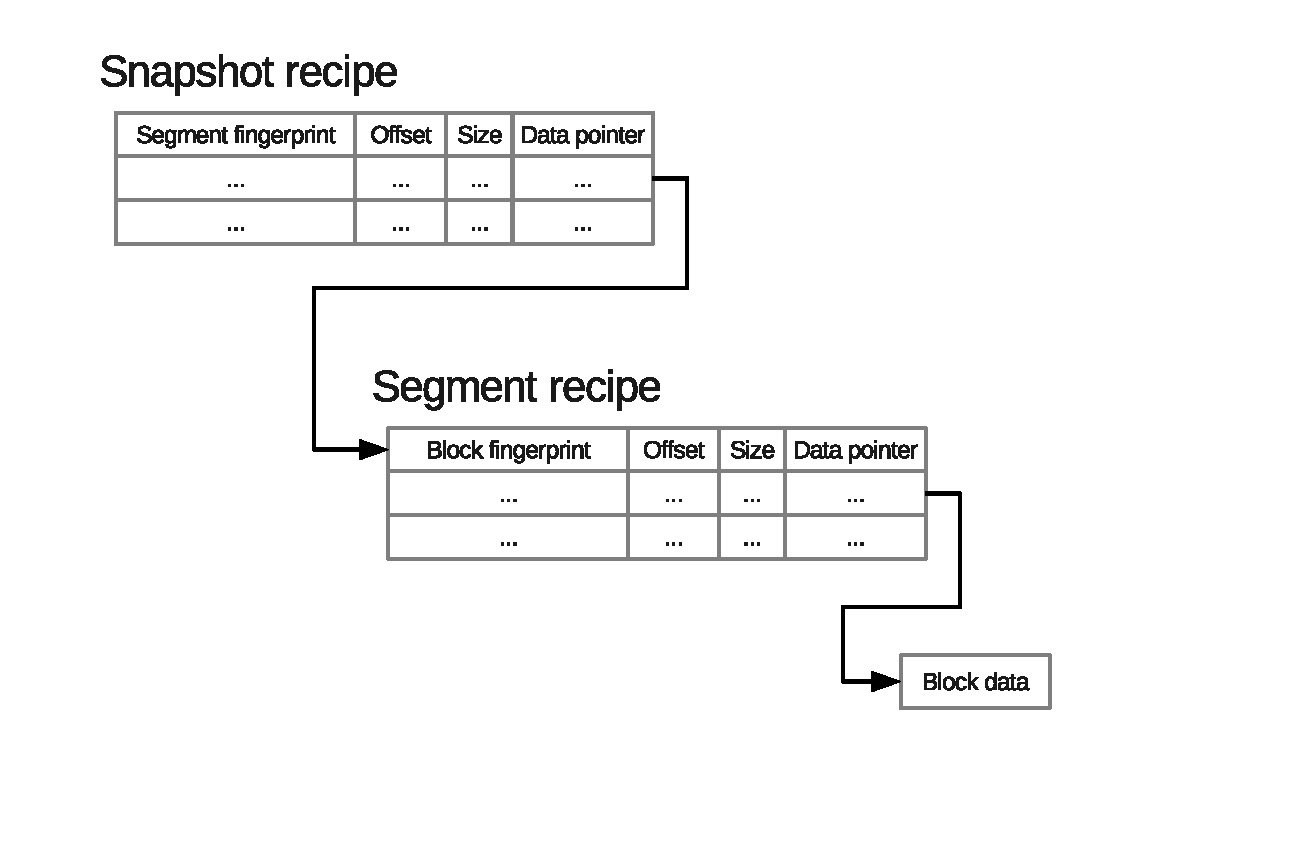
\epsfig{file=images/snapshot_representation, width=3in}
%  \caption{An example of snapshot representation.}
%  \label{fig:snapshot_rep}
%\end{figure}
%As a result, the representation of each snapshot is designed as a two-level index data structure 
%in the form of a hierarchical directed acyclic graph as shown in Figure \ref{fig:snapshot_rep}.
%A snapshot recipe contains a list of segments, each of which is represented as a segment recipe
%that holds the meatdata of its chunks. We choose this two-level structure because in practice we
%observe that during each backup period only a small amount of VM data are added or modified. 
%As the result, even the metadata of two snapshots can be highly similar, 
%thus aggregating a large number of chunks as one segment can significantly reduce the space cost of snapshot metadata.
%Furthermore, instead of using variables-sized segments, we use a dirty bit to capture the change status of fix-sized
%segments which greatly ease the segment-level deduplication.
In snapshot and segment recipes, 
the data structures  includes reference pointers to the actual data location to eliminate the need for additional indirection.
%In our implementation the data reference is a 8 bytes field which is either an 
%ASID (discuss in Section \ref{sect:append}) or an offset of an additional flag indicates
%the location of PDS data.





%\subsection{Snapshot management}


\begin{figure*}[t]
    \centering
    \includegraphics[width=6in]{images/socc_arch_cluster}
    \caption{System Architecture}
    \label{fig:arch_vm}
\end{figure*}

\comments{%socc_arch_cluster now includes the entire arch instead of having 2 figures
\begin{figure}
    \centering
    \subfigure[Node architecture from VM point of view]
    {
        \includegraphics[width=3in]{images/socc_arch_vm}
        \label{fig:arch_vm}
    }
    \\
    \subfigure[Cluster architecture]
    {
        \includegraphics[width=3in]{images/socc_arch_cluster}
        \label{fig:arch_cluster}
    }
    \caption{System architecture.}
    \label{fig:arch}
\end{figure}
}

%[describe the architecture frm node side]
%[brief the virtual device driver]
%One physical node hosts tens of VMs, each of which access its virtual machine disk image through the
%virtual block device driver (called TapDisk\cite{Warfield2005} in Xen).
%This driver maintains a map of dirty-bits to record
%the change status of every fix-size segment of the virtual disk. 
%When the VM issue a disk write, the bits coresponding to the segments that covers 
%the modified disk region are set, thus letting snapshot deduplication component knows these
%segments must be checked during snapshot backup. After the snapshot backup is finished, 
%snapshot deduplication component acknowledges the driver to resume the dirty-bits map to
%a clean state.

%[brief the snapshot deduplication]
%The snapshot deduplication component consists of the chunking and deduplication 
%logic of our snapshot storage system. We choose 

%[describe the arch from cluster side]


%[describe the data structure in underlying storage]
\subsection{A VM-centric snapshot store for backup data}

We build the snapshot storage on the top of a distributed file system.
Following the VM-centric idea for the purpose of fault isolation,
each VM has its own snapshot store, containing new data chunks which are considered
to be non-duplicates.
There is also a special store containing all PDS chunks shared among different VMs.
% with a higher replication degree.
%This separation of PDS chunks allows us to change the replication degree of of those popular file blocks in the 
%underlying file system
%Extra replication of this store is added and analyzed in Section~\ref{sect:analysis}.
As shown in Fig.\ref{fig:as_arch}, we explain the data structure of snapshot stores as follows.

\begin{itemize}

%The reference to each PDS cunk  contains  a container ID as explained ,   

%The PDS index uses the offset and size as a reference in its index structure.
 
\item Data of each VM snapshot store excluding PDS is divided into a set of containers and 
each container is approximately 1GB. 
The reason for dividing the snapshot into containers is to simplify the compaction process
conducted periodically. As discussed later, data chunks are deleted from old snapshots
and chunks without any reference from other snapshots can be removed by this compaction process.
By limiting the size of a container, we can effectively control the length of each compaction process.
The compaction  routine can work on one container at a time and copy used data chunks to another container. 


Each container is further divided into a set of chunk data groups. Each chunk group is composed of
a set of data chunks and is the basic unit in data access and retrieval. 
In writing a chunk during backup, the system accumulates data chunks and store the entire
group as a unit after a compression.
When accessing a particular chunk, its chunk group is retrieved from the storage
and uncompressed. Given the high spatial locality and usefulness of prefetching  in 
snapshot chunk accessing~\cite{Sampling,FoundationPaper},
retrieval of  a data chunk  group naturally works well with prefetching. 
A  typical chunk group contains 100 to 1000 chunks, with an average size of 
200-600 chunks.
%Given  the average chunk size of 4KB,  the index size for a 1GB container reduces from 10MB to 100KB when
%the chunk group size is 100.
%%CBlock, then the overall index size is reduced to $1/m$. 
%n our implementation, using $m=100$ reduces the index for
%a 1GB container from 10 MB to 100 KB.
\item Each data container is represented by three files in the DFS:
1) the container data file holds the actual content, 
2) the container index file is responsible for translating a data reference
into its location within a container, and 
3) a chunk deletion log file records all the deletion requests within  the container.

%A VM snapshot store typically has a small number of containers because each container is 
%fairly large, with an average size of 1GB, and 
%maintains a limited number of snapshots (e.g. 10 in the Alibaba case).
%New snapshot data chunks can be effectively compressed in chunk groups in addition to  deduplication.

\item A data chunk reference stored in the index of snapshot recipes
is composed of two parts: a container ID with 2 bytes and a local chunk ID with 6 bytes.
Each container maintains a local  chunk counter and assigns the current number 
as a chunk ID  when  a new chunk is added to this  container. 
Since data chunks are always appended to a snapshot store during backup, 
a local chunk ID is monotonically increasing.
When a snapshot chunk is to be accessed, the recipe for the snapshot will point a data chunk
in the PDS store or in a non-PDS VM snapshot  store. 
Using  a container ID, the corresponding container index file of this VM is accessed and 
the chunk group is identified using a simple chunk ID range search. Once the chunk group is loaded to memory, 
its header contains the exact offset of the corresponding chunk ID and the content is then accessed from the memory buffer.

%Every container  Store assign every piece of data a CID for its internal data referencing. 
%When new data is appended, its CID is the current largest CID in that container plus one.
%As a result, all the data locations are naturally indexed by this self-incremental CID, 
%no extra sorting is needed.
\item The PDS chunks are a set of commonly used data and they are stored in one PDS file.
Since the total file size is relatively small, and
PDS data is re-calculated periodically, the PDS data file and its index are rebuilt completely. 
Each reference to a PDS data chunk in the PDS index is the offset within the PDS file, and the chunk size.

\end{itemize}

%acceretrieved  and ret
%Using CBlock brings us several advantages: First, the write workload to DFS master is greatly reduced; second, grouping
%small chunks gives better compression. Third, reading a CBlock (200 - 600 KB) typically cost the same amount of disk 
%seek as reading a 4KB chunk. Finally, this greatly reduces the size of index. Let $m$ be the number of chunks in each
%CBlock, then the overall index size is reduced to $1/m$. In our implementation, using $m=100$ reduces the index for
%a 1GB container from 10 MB to 100 KB.

 
% of  divided into a set of data containers.
%Each container has 3 parts.
%Each chunk in the snapshot is referenced by the following data format

%The Append Store (AS) is our underlining storage engine for storing snapshot data in the distributed file system
%after deduplication.
%AS is built on top of our highly scalable distributed file system (DFS), 
%which is very similar to Google's file system
%in a sense that it is optimized for large files and sequential read/append operations.

\begin{figure}[htbp]
  \centering
  \epsfig{file=images/sstore_arch, width=3in}
  \caption{Data structure of a VM snapshot store.}
  \label{fig:as_arch}
\end{figure}

%\begin{figure}[htbp]
%  \centering
%  \epsfig{file=images/pds_arch, width=3in}
%  \caption{System architecture for PDS data store.}
%  \label{fig:as_arch}
%\end{figure}

A snapshot  store supports three API calls.
\begin{itemize}

%AS supplies three interfaces: {\em get(ref)} accepts a data reference and retrieves data, 
\item {\em Put(data)}. This places data chunk into the snapshot store and returns a reference to be stored in 
the recipe metadata of a snapshot. 
The write requests to append data chunks to a VM store are accumulated at the client side. 
When the number of write requests reaches a fixed group size, the snapshot store client compresses
the accumulated   chunk group, adds a chunk group index  to the beginning of the group, and then
appends the header and data  to the corresponding VM file.
A new container  index entry is also created for each chunk group and is written the corresponding
container index file.
The writing of PDS data chunks is conducted periodically when there is a new PDS calculation.
%Since the PDS dataset is small, a new PDS file is created during the periodical update.
\item{\em Get(reference)}.
The fetch operation for the PDS data chunk is straightforward since each reference contains 
the offset and size within the PDS  underlying  file.
We also maintain a small data cache for the PDS data service to speedup common data fetching.

To read a non-PDS chunk using its reference with container ID and local chunk ID,  the snapshot store client first loads the
corresponding VM's container index file specified by the container ID, then searches the chunk
groups  using their  chunk ID coverage.
After that, it reads the identified chunk group from DFS, decompresses it, and seeks to the exact chunk data 
specified by the chunk ID. 
Finally, the client updates its internal chunk data cache with the newly loaded content to 
anticipate future sequential reads.
\item {\em Delete(reference)}.
Chunk deletion occurs when a snapshot expires or gets deleted explicitly by a user
and we will discuss the snapshot deletion in detail in the following subsection.
%deletes the data pointed by the reference.
%Under the hood, small var-sized data are grouped and stored into larger data containers. Each VM has
%its snapshot data stored in its own Append Store, specified by the VM ID. 
%We split every Append Store into multiple data containers so that reclaiming the disk space would not 
%result in rewriting all the data at the same time.
When deletion requests are issued for a specific container,
those requests are simply recorded into the  container's deletion log initially and thus  a lazy
deletion strategy is exercised.
Once local chunk IDs appear in
the deletion log, they will not be referenced by any future snapshot and can be safely deleted when needed. 
Periodically, the snapshot  store picks those containers with an excessive
number of deletion requests to  compact and  reclaim the corresponding disk space. 
%The actual compaction will only take place when the number of deleted items 
%reached $d\%$ of container's capacity. 
During compaction, the snapshot store creates a new container (with the same container ID) to replace the 
existing one. This is done by sequentially scanning the old container, copying all the chunks that are not 
found in the deletion log to the new container, and creating new chunk groups and indices. 
Every local chunk ID however is directly copied rather than re-generated. This
process leaves holes in the CID values, but preserves the sorted order.
As a result, all data references stored 
in upper level recipes are permanent and stable, and the data reading process
is as efficient as before. Maintaining the stability of chunk IDs also ensures that recipes do not
depend directly on physical storage locations.
\end{itemize}

%As shown in Fig.\ref{fig:as_arch}, every data container is represented as three data files in DFS:
%the data file holds all the actual data, the index file is responsible for translating data reference
%into data locations, and a deletion log file remembers all the deletion requests to the container.
%
%A data reference is composed of two parts: a container ID (2 bytes) and CID (6 bytes).
%Append Store assign every piece of data a CID for its internal data referencing. 
%When new data is appended, its CID is the current largest CID in that container plus one.
%As a result, all the data locations are naturally indexed by this self-incremental CID, 
%no extra sorting is needed.

%Append Store groups multiple chunk data (i.e., 100) into larger units, called {\em CBlock}.
%CBlock is the basic unit for append store's internal read/write/compression.
%There is one index entry in the container index corresponding to every CBlock. It keeps the first chunk's CID
%in that CBlock, and the CBlock data's size and location.
%
%Using CBlock brings us several advantages: First, the write workload to DFS master is greatly reduced; second, grouping
%small chunks gives better compression. Third, reading a CBlock (200 - 600 KB) typically cost the same amount of disk 





\subsection{ VM-centric Approximate Snapshot Deletion with Leak Repair}

\begin{figure}[htbp]
  \centering
  \epsfig{file=images/deletion.png, width=3.5in}
  \caption{Approximate deletion}
  \label{fig:deletion_flow}
\end{figure}

In a busy VM cluster, snapshot deletions can occur frequently.
Deduplication complicates the deletion process because space saving relies on the sharing of data
and it requires the global reference of deleted chunks to be identified before  they can be safely removed.
While we can use the mark-and-sweep technique~\cite{Guo2011}, 
it still takes significant resource to conduct this process every time there is a snapshot deletion.
In the case of Alibaba, snapshot backup is conducted automatically and there are 
about 10 snapshot stored for every user. When there is
a new snapshot created every day,  there will be  a snapshot expired everyday to maintain
a balanced storage use. 

%Given the large number of snapshot deletion requests, 
We seek a fast solution with a low resource usage to delete snapshots.
%In a traditional deduplication system, deletion often require looking at global scope to
%resolve the data dependency between logical backup entities and physical data chunks.
Our VM-centric snapshot storage design simplifies the deletion process since 
we can focus on  unreferenced chunks within each VM.
The PDS data chunks are commonly shared all VMs and we do not consider them
during snapshot deletion.  The selection of PDS data chunks is updated periodically independent of snapshot deletion process.
Another resource-saving strategy we propose is
an {\em approximate} deletion strategy to trade deletion accuracy for
speed and resource usage. Our method sacrifices a small percent of storage leakage
to efficiently identify unused chunks.
% in $O(n)$ time where $n$ is the total number of non-PDS chunks to be deleted from a VM snapshot store.  
The algorithm contains three aspects.


%Our system adopts VM-centric snapshot  lazy delete strategy so that all snapshot deletions are scheduled
%in the backup time window at midnight. 
%Therefore, snapshot deletions must be fast enough to fit in time window and
%efficient enough to satisfy our resource constraints.
%However, there is no simple solution can achieve these goals with high reliability.
%Our hybrid deletion strategy, using fuzzy deletion regularly and accurate deletion periodically,
%accomplishs our speed, resource usage and relibility goals very well.
\begin{itemize}
\item {\bf Computation for snapshot fingerprint summary.}
Every time there is a new snapshot created,
we compute a bloom-filter with $z$ bits as the summary of reference pointers for all non-PDS chunks used 
in this snapshot. Given $h$ snapshots stored for a VM, there are $h$ summary vectors maintained.

%To control the false positive ratio $\epislon$ under $0.01$, an average snapshot of size 40 $GB$ with 
%$u \approx 10$ million chunks, $z$ has 10 million bits. 

%{\bf Creating bloom filter} Scan all the living snapshot recipess and their segment recipes,
%for every reference pointing to append store, add it to the bloom filter.

\item {\bf Approximate deletion with fast summary comparison.}
When there is a snapshot deletion,  
we need to identify if  chunks to be deleted from that snapshot
are still used by other snapshots. 
This is done approximately and quickly by comparing the 
reference pointers of deleted snapshot with
the merged reference bloom-filter summary of other live snapshots.
The merging of live snapshot bloom-filter bits uses the logical OR operator 
and the merged vector still takes $z$ bits.
Since the number of live snapshots $h$ is limited for
each VM, 
the time and memory cost of this comparison is small, linear to the number of chunks to be deleted.
%Instead of scanning the entire append store indices, we merge the type-1 summaries of all
%valid snapshots. 
%Since each VM has uniform bloom filter parameters to create snapshot summaries, 
%such merged summeries give us a compact representation of
%all block fingerprints that are still in use.
%Thus by the property of bloom filter, if a fingerprint is not found in merged summaries, 
%we are certain that block is no longer used by any valid snapshot, it would be then added
%to append store's deletion log.

If a chunk's reference pointer is not found in the merged summary vector, we are sure that
this chunk is not used by any live snapshots, thus it's safe delete it. 
However, among all the chunks to be deleted, 
there is a small percentage of unused chunks  which
are misjudged as  being in use, resulting in a storage leakage.


\item {\bf Periodic repair of leakage}.
%[exlpain why second bloom filter, why scan append store]
%Since there are certain unused chunks which are not deleted during the approximate deletion, 
Leakage repair is conducted periodically to fix the above approximation error.
This procedure compares the live chunks for each VM with what are truly used through the VM snapshot metadata recipe.
That requires a scanning of all chunks in a VM; however it is a VM-specific procedure and thus
the cost is relatively small compared to the traditional mark-sweep procedure~\cite{?} which scans snapshot 
chunks from all VMs.
For example,
% are live used   we load the reference pointers of all chunks from a VM snapshot store as a table in memory,
%then scan through all the snapshots' segment recipes. For each reference pointer that is in use by a snapshot,
%we mark the corresponding entry in the table as in use. Finally those unmarked (and therefore unused) reference pointers in the
%table represent chunks that can be safely deleted.
%The cost of leak repair mainly come from holding a table of reference pointers and the scan of all snapshots' metadata.
consider each reference pointer consumes 8 bytes plus  1 mark bit, a VM that has 40GB backup data with about
10 million chunks will need less than 90MB of memory to complete a VM-specific mark-sweep process.
%, scanning all snapshots metadata is many times slower when compared
%to the approximate deletion which only scans single snapshot's metadata.
%It's worth mention that compared to previously-developed mark-and-sweep techniques, 
%our leak repair still has advantages because the scope of repair is restricted within a single VM's snapshot 
%store due to our VM-centric design, and we perform leakage repair periodically.
%We cannot simply repeat the phase 1 multiple times to reduce temporary storage leakage, because:
%\begin{enumerate} 
%\item After several runs of phase-1, it is proven that the merged type-1 summaries cannot sieve remaining unused blocks, due to the false-positive property of bloom filter.
%\item The recipes of deleted snapshots have been removed from the system, thus we are not able to obtain the deleted block fingerprints from any metadata, the only way to discover them is to scan the append store indices.
%\end{enumerate}
\end{itemize}




%\item {\bf Check existance} For every data reference in the deleted snapshot recipe and its segment recipes,
%check the existance of that data reference in bloom filter. If not found, it is safe to delete that piece of data from append store
%because no living snapshots has referenced it.

%The overall time of running a approximate deletion for one snapshot deletion would be scanning
%all the living snapshots and deleted snapshots, since operations on the in-memory bloom filter can be done in
%parallel and is much faster than loading recipes from DFS:
%\begin{equation}
%T = (N_{SS} + 1) * T_{scan\_recipes}
%\end{equation}
%
%Using the example and analysis in previous section, this approximate deletion can be done in 5 minutes.
%Memory usage of the bloom filter depends on its false-positive probility $P_{bl}$,
%when set $P_{bl}$ to 0.01, the memory footprint of approximate deletion is about 15 MB.
%~



%{\bf Discussion}
We now estimate the size of storage leakage and how often leak repair needs to be conducted,
given  a VM which keeps $h$ snapshots in the backup storage, and it creates and deletes one snapshot
everyday. Let $u$ be the total number of chunks brought by the initial backup, $\Delta u$ be the average
number of additional unique chunks added from one snapshot to the next snapshot version. Then the total number of unique
chunks used in a VM is about:
\[
U = u + (h-1)\Delta u.
\]

Each bloom filter vector has  $z$ bits for each snapshot and let $j$ be the number of hash functions used by the
bloom filter. The probablity that a particular bit is 0  in all $h$ summary vectors is  
$(1- \frac{1}{z}) ^{j U}$. Notice that a chunk may appear multiple times in these summary vectors; however, this should not 
increase the probability of being a 0 bit in all $h$ summary vectors.
Then the misjudgment rate of being in use $\epsilon$ is: 
\begin{equation}
\label{eq:falserate}
\epsilon = (1-(1-\frac{1}{z})^{jU})^j.
\end{equation}


For each snapshot deletion, the amount of chunks need to be deleted is nearly identical to the number of
newly add chunks $\Delta u$. 
%However, some of chunks among them are not detected as unused in our approximation
%algorithm, thus forms the storage leakage. 
Let $R$ be the total number of runs of approximate deletion between two consecutive 
repairs. we estimate  the total leakage $L$ after $R$ runs as:
\[
L = R \Delta u \epsilon
\]

When leakage ratio $L/U$ exceeds a pre-defined threshold $\tau$, we need to execute a leak repair:

\begin{equation}
\label{eq:leakrepair}
\frac{L}{U} = \frac{R \Delta u \epsilon}{u+(h-1)\Delta u } > \tau 
\Longrightarrow R > \frac{\tau}{\epsilon}\times\frac{u + (h-1)\Delta u}{\Delta u}
\end{equation}

For example in our tested dataset,  
each VM keeps $h=10$ snapshots and each snapshot has
about 1-5\% of new data. Thus $\frac{\Delta u}{u} \leq 0.05$. For a 40GB snapshot, $u\approx  10$ millions.
Then $U=10.45$ millions.
We choose  $\epsilon = 0.01$ and $\tau=0.1$.  From Equation~\ref{eq:falserate}, 
$z=10U=100.45$ million bits. From Equation~\ref{eq:leakrepair}, 
leak repair should be triggered once for every R=290 runs of approximate deletion. 
When one machine hosts 25 VMs and there is one snapshot deletion per day per VM, there would be 
only one full leak repair for one VM scheduled for every 12 days. Each repairs uses at most  90MB memory on average
as discussed earlier and takes a short period of time.
% which is sufficiently small to offset the heavy I/O workload of the mark-sweep process.
